%!TEX program = pdflatex

\documentclass[a4paper, 12pt]{article}

\usepackage{geometry}
\geometry{a4paper,
total={170mm,257mm},left=2cm,right=2cm,
top=1cm,bottom=2cm}

\usepackage{mathtext}
\usepackage{amsmath}
\usepackage[T2A]{fontenc}
\usepackage[utf8]{inputenc}
\usepackage[english,russian]{babel}
\usepackage{graphicx, float}
\usepackage{tabularx, colortbl}
\usepackage{caption}
\captionsetup{labelsep=period}

\newcommand{\parag}[1]{\paragraph*{#1:}}
\DeclareSymbolFont{T2Aletters}{T2A}{cmr}{m}{it}
\newcounter{Points}
\setcounter{Points}{1}
\newcommand{\point}{\arabic{Points}. \addtocounter{Points}{1}}
\newcolumntype{C}{>{\centering\arraybackslash}X}

\begin{document}
%\maketitle

\begin{titlepage}
    \vspace*{\fill}
    
    \begin{center}
        
\includegraphics[scale=0.8]{res/MIPT.pdf}
        \\[0.7cm]\Huge Московский Физико-Технический Институт
        \\[2cm]\LARGE Отчет о выполнении лабораторной работы 
        \\[0.5cm]\noindent\rule{\textwidth}{1pt}
        \\\Huge\textbf{5.8.1 \\ Определение постоянных Стефана-Больцмана и Планка из анализа теплового излучения накаленного тела}
        \\[-0.5cm]\noindent\rule{\textwidth}{1pt}
    \end{center}
    
    \vspace*{\fill}
    
    \begin{flushleft}
        Выполнили: \hspace{\fill} Группа:
        \\Костылев Владислав \hspace{\fill} Б01-206
    \end{flushleft}
\end{titlepage}

\setcounter{page}{2}


\begin{abstract}
    \textbf{Цель работы:} 
        При помощи модели абсолютно чёрного тела проведение измерения температуры оптическим пирометром с исчезающей нитью и термопарой.
        Исследование излучение накалённых тел с различной испускательной способностью.
        Определение постоянных Планка и Стефана-Больцмана
    
    \textbf{В работе используются:} 
        Оптический пирометр, модель абсолютно чёрного тела, образцы колец, вольфрамовая лампа, неоновая лампа, блок питания, цифровые вольтметры
\end{abstract}

\tableofcontents
\newpage

\section{Теоретическая справка} 

    Для измерения температуры разогретых тел, удалённых от наблюдателя, применяют методы оптической пирометрии, 
    основанные на использовании зависимости испускательной способности исследуемого тела от температуры. 
    Различают три температуры, функционально связанные с истинной термодинамической температурой и излучательной способностью тела: 
    радиационную $T_{rad}$, цветовую $T_{col}$ и яркостную $T_{br}$. \par
    В работе измеряется яркостная температура. \textbf{Яркостная температура} - это температура 
    абсолютно чёрного тела, при которой его спектральная испускательная способность равна спектральной испускательной 
    способности исследуемого тела при той же длине волны.
    Измерение яркостной температуры раскалённого тела производится при помощи оптического пирометра с исчезающей нитью, 
    основанного на визуальном сравнении яркости раскалённой нити с яркостью изображения исследуемого тела. \par
    Яркостная температура тела всегда ниже его термодинамической температуры. Это связано с тем, 
    что любое нечёрное тело излучает меньше, чем АЧТ при той же температуре. Зависимость между яркостной и 
    термодинамической температурами вольфрама приведена на рисунке ниже:

    \begin{figure}[H]
        \centering
        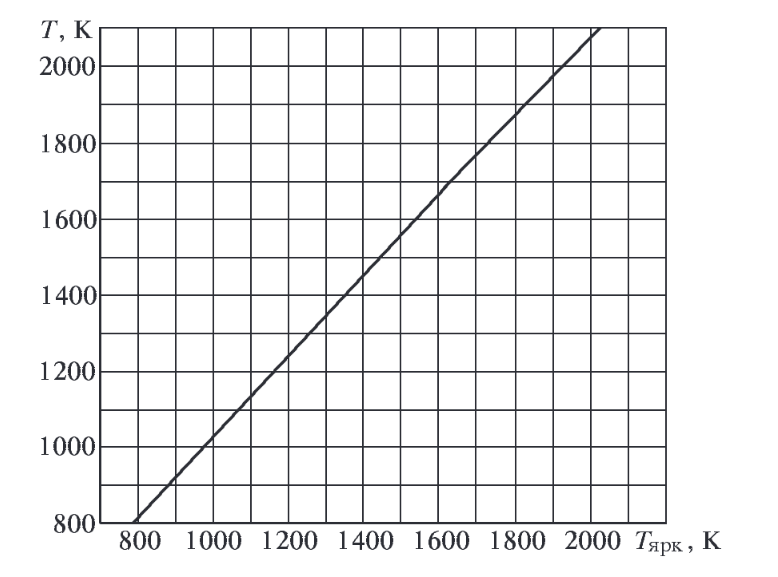
\includegraphics[width=0.7\linewidth]{res/1.png}
    \end{figure}

    По результатам измерений мощности излучения вольфрамовой нити можно судить о справедливости 
    закона Стефана-Больцмана. Если бы нить излучала как АЧТ, 
    то баланс потребляемой и излучаемой энергии определялся бы соотношением:
    \begin{equation}
        W = \sigma S (T^4 - T_0^4),
    \end{equation} 
    
    где $W$ - потребляемая нитью электрическая мощность, $S$ - площадь излучающей поверхности нити, 
    $T$ - температура нити, $T_0$ - температура окружающей среды. 
    Однако вольфрамовая нить излучает как серое тел, и излучение её ослаблено по сравнению с АЧТ 
    в $\varepsilon_T$ раз для любой волны при данной температуре тела Т. 
    Тогда предположив, что нить излучает как серое тело и с учётом того, что $T_0 \ll T$, выражение (1) можно переписать в виде
    
    \begin{equation}
        W = \varepsilon_T S \sigma T^4
    \end{equation}

    В справедливости закона Стефана-Больцмана можно убедиться, построив график зависимости $W(T)$ в 
    логарифмическом масштабе и по углу наклона определить показатель степени $n$ исследуемой    температурной зависимости. 
    В пределах погрешности показатель степени должен быть близок к четырём. \par
    Также из формулы (2) можно определить постоянную Стефана-Больцмана.

    \section{Экспериментальная установка}

    \begin{figure}[H]
        \centering
        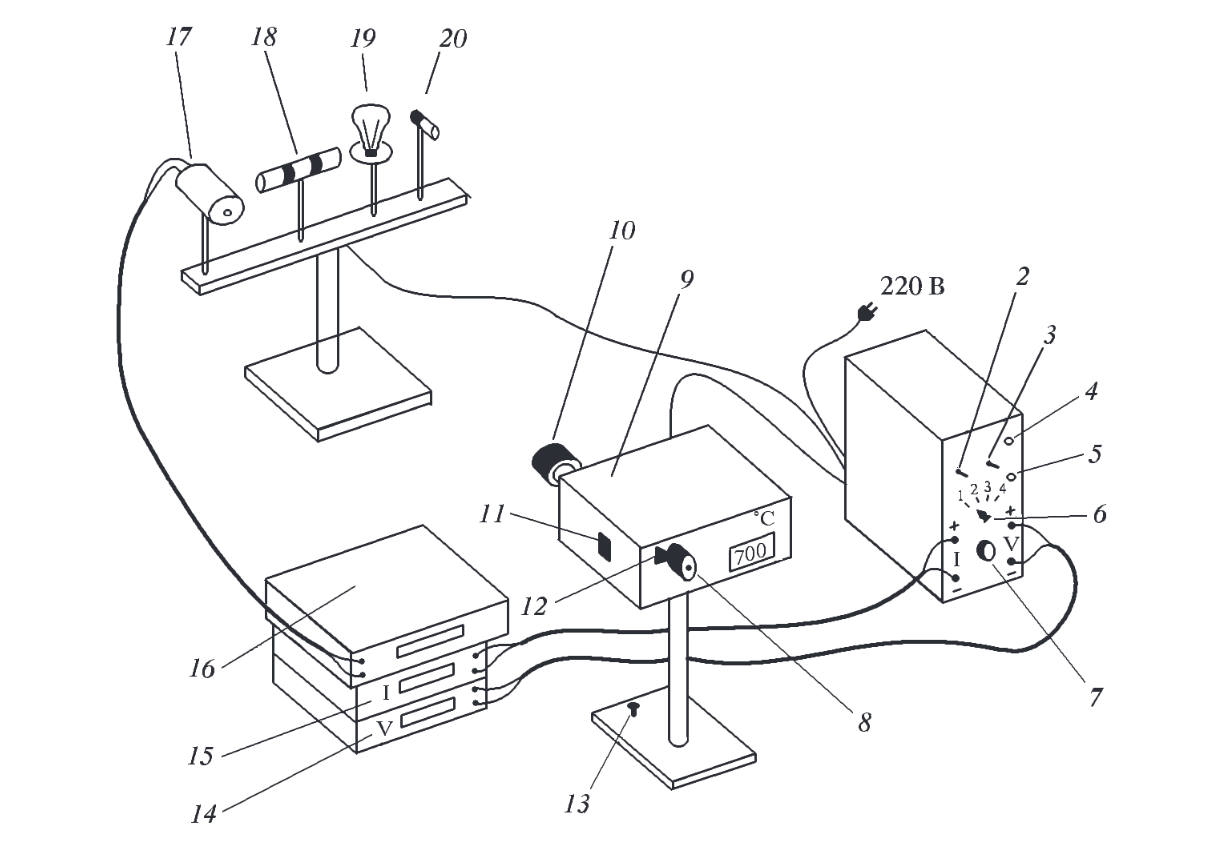
\includegraphics[width=0.7\linewidth]{res/2.png}
    \end{figure}

    Исследуемые в работе образцы:
    \begin{itemize}
        \item \textbf{модель абсолютно чёрного тела} - керамическая трубка, закрытая 
        с одного конца и окружённая для теплоизоляции внешним кожухом. 
        Температура в трубке измеряется с помощью термопары хромель-алюмель
        \item \textbf{керамическая трубка с набором колец из различных материалов}, 
        нагреваемая изнутри нихромовой спиралью. Материалы колец имеют различную излучательную способность
        \item \textbf{вольфрамовая нить электрической лампочки}
    \end{itemize}

% \section {Методика измерений}
    

\section{Результаты измерений и обработка данных} 

    \begin{figure}[H]
        \centering
        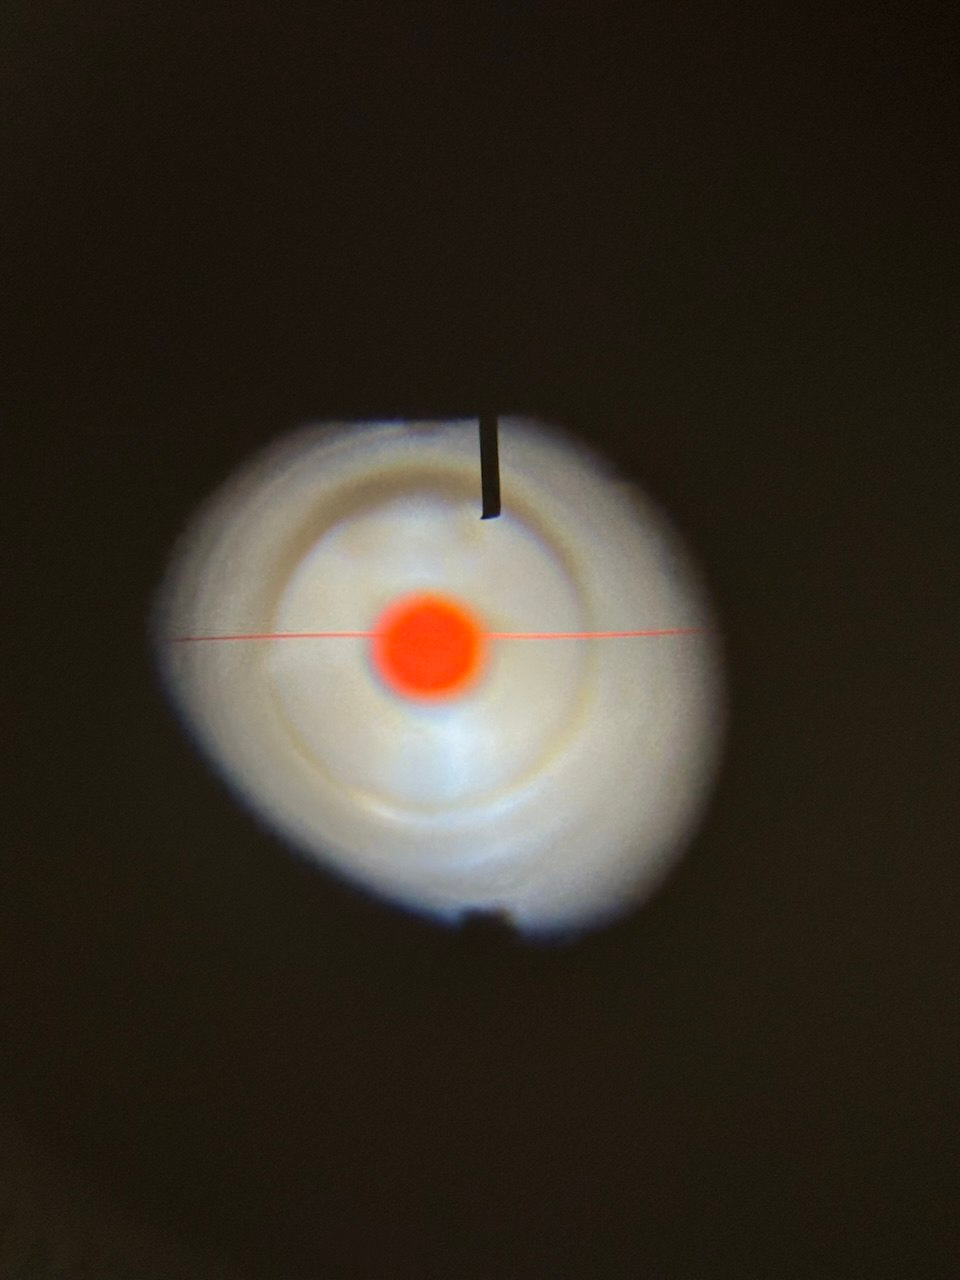
\includegraphics[width=0.4\linewidth]{res/5.png}
    \end{figure}

    \begin{figure}[H]
        \centering
        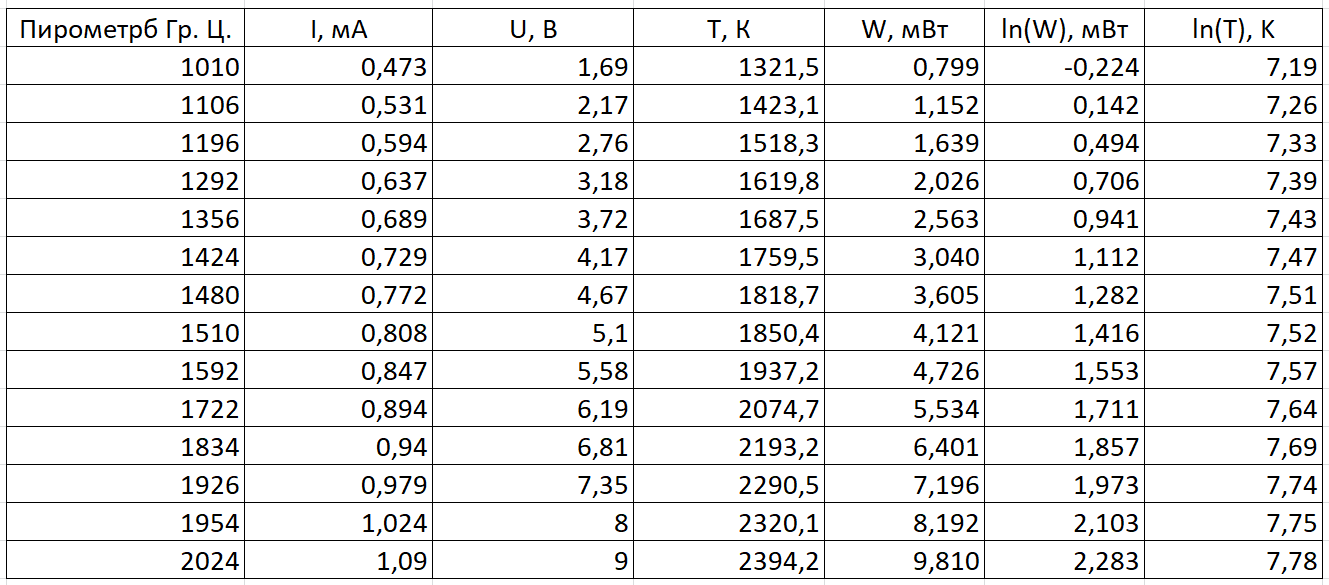
\includegraphics[width=0.7\linewidth]{res/3.png}
    \end{figure}

    После обработки наших результатов, построим график в логарифмическом масштабе, 
    для проверки закона Стефана-Больцмана:
    \begin{figure}[H]
        \centering
        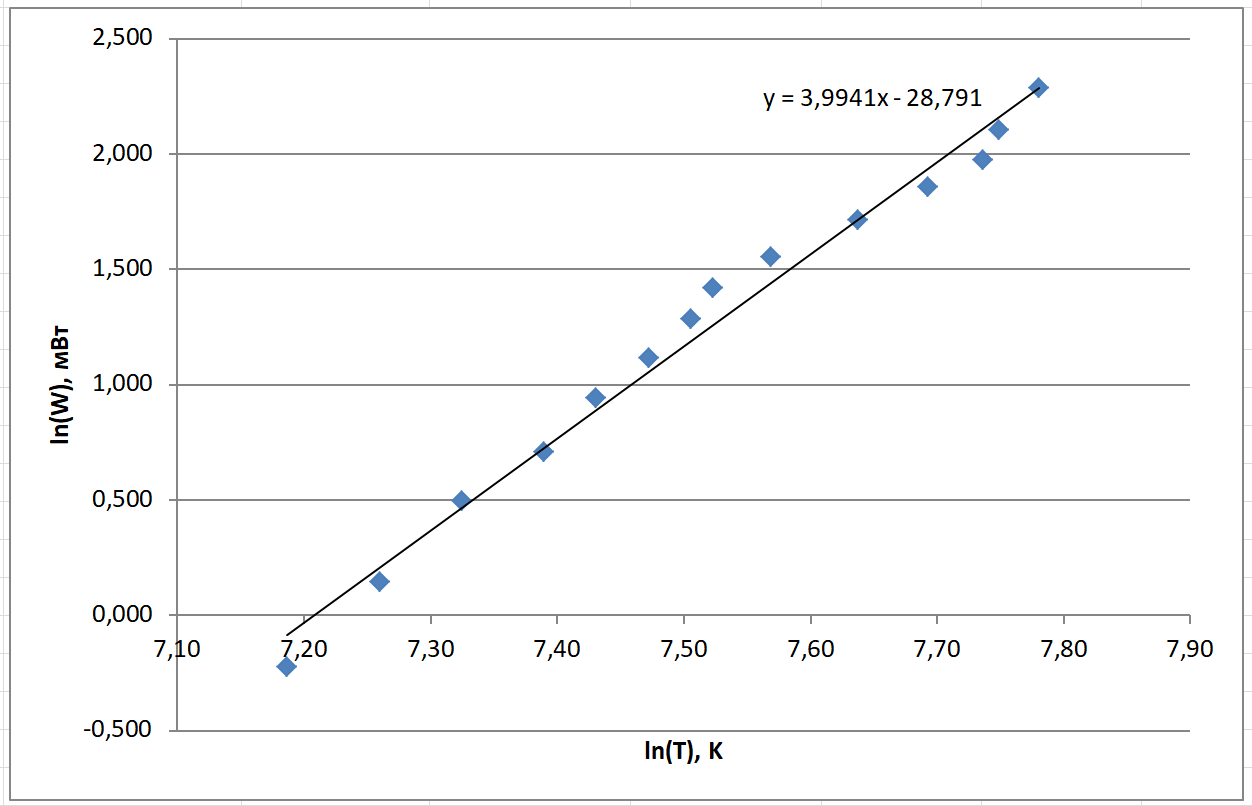
\includegraphics[width=0.7\linewidth]{res/4.png}
    \end{figure}

    Уравнение имеет следующий вид:
    \[
        \ln W = \ln(\varepsilon_{T} \sigma S) + n*\ln T
    \]
    где $S = 0,36 см^2$ - эффективная площадь излучающей поверхности нити. \\

    Исходя из графика получаем n примерно равное 4 (как и должно быть). \\

    Теперь вычислим постоянную Стефана-Больцмана для температуры 2074 К ($\varepsilon = 0,252$): 
    \[ 
        \sigma = \frac{W}{\varepsilon_{T} S T^4} = \frac{5,534 * 10^{-3}}{0,252 * 0,36 * 10^{-4} * 2074^{4}} = 3,3 * 10^{-11} Вт*м^{-2}*K^{-4}
    \]

    Что к сожалению не сходится с теоретическим значением на 3 порядка ($\sigma = 5,67 * 10^{-8} Вт*м^{-2}*K^{-4}$).

    Также можно определить постоянную Стефана-Больцмана, используя построенный график зависимости $\ln(W) = \ln(\varepsilon_T \sigma S) + n \ln(T)$
    \[    
        \ln(\varepsilon_t \sigma S) = -28.791
    \]
    \[
        \sigma = \frac{e^{-28.791}}{\varepsilon_T S} = 3.46*10^{-8} Вт*м^{-2}*K^{-4}
    \]

    Что уже очень близко к теоретическому значению. \\

    Оценим значение постоянной Планка:
    \[
        h = \sqrt[3]{\frac{2 \pi^5 k_B^4}{15 c^2 \sigma}} = \sqrt[3]{\frac{2 *3,14^5*(1,38*10^{-23})^4}{15*(3*10^8)^2*3.46*10^{-8}}} = 
        \sqrt[3]{\frac{100*2*3,14^5*1,38^4}{15*3*3.46}}*10^{-34} = 11,25*10^{-34} Дж*с
    \]

    Что очень близко к теоретическому значению: 
    \[ 
        h_{th} = 6,62 * 10^{-34} Дж*с
    \]

    \subsection{Измерение яркостной температуры неоновой лампочки}
    Термодинамическая температура неоновой лампочки примерно равна комнатной, 
    и не соответствует её яркостной температуре ($\approx$ 904$^{\circ}$C). 
    Дело в том, что неоновая лампочка в принципе не является моделью абсолютно чёрного или 
    серого тела, и её излучение носит совершенно другую природу (переход электронов между энергетическими уровнями). 
    То, что её свет имеет такой же цвет, что и нагретое АЧТ - совпадение.


\section{Заключение}
    В заключение могу отметить, что мы при помощи модели абсолютно чёрного тела провели измерения температуры оптическим пирометром с исчезающей нитью и термопарой.
    Исследовали излучение накалённых тел с различной испускательной способностью и определили постоянные Планка и Стефана-Больцмана, хоть и не с очень большой точностью.
    
\end{document}
